%//////////////////////////////////
%/// P R E A M B L E

\documentclass[a4paper, 12pt]{article}

\usepackage{geometry}
\usepackage[utf8]{inputenc}
\usepackage[singlespacing]{setspace}
\usepackage{amsmath}
\usepackage{mathtools}
\usepackage{caption}
\usepackage{float}
\usepackage{booktabs}
\usepackage{graphicx}
\usepackage{multicol}
\usepackage{gensymb}
\usepackage{breqn}
\usepackage{indentfirst}
\usepackage{siunitx}
\usepackage{tabularx, booktabs}
\usepackage[calcwidth]{titlesec}
%\newcolumntype{Y}{>{\centering\arraybackslash}X}
\usepackage{xcolor}
\usepackage{pdfpages}

\usepackage{multicol}
%\usepackage{supertabular}

\usepackage{svg}

\widowpenalty = 4500
\clubpenalty  = 4500

\newcommand*\dif{\mathop{}\!\mathrm{d}}
\newcommand*\shortminus{\scalebox{0.5}[1.0]{\( - \)}}
\newcommand{\hspa}{\hspace{0.02128623625220817\paperwidth}}
\newcommand{\hspb}{\hspace{0.013155617496424828\paperwidth}}

\definecolor{hsblue}{HTML}{0cb5df}
\definecolor{hsblueshade}{HTML}{b6e9f5}

\setlength{\jot}{0.013155617496424828\paperheight}

%%========================================
%% circuitikz properties
\usepackage[european, straightvoltages]{circuitikz}
%\ctikzvalof{voltage/distance from node = .2}
%\ctikzset{voltage/distance from node  =.5}% in \pgf@circ@Rlen units
%\ctikzset{voltage/distance from line  =.25}% pos. between 0 and 1
%\ctikzset{voltage/bump b/.initial     =1.5}%

\ctikzset{current/distance            = .618}


%%========================================

%%
%% Path settings
%%
\graphicspath{ {./graphics/} }

\geometry{
 a4paper,
 total={0.6180339887498948\paperwidth,0.6180339887498948\paperheight},
 top = 0.1458980337503154\paperheight,
 bottom = 0.1458980337503154\paperheight
 }

\linespread{1.1458980337503154}

\titleformat{\section}[hang]{\Large\bfseries}{\thesection\hspb\textcolor{hsblueshade}{|}\hspa}{0pt}{\Large\bfseries}

\setlength{\parskip}{0.013155617496424828\paperheight} % paragraph spacing

\titlespacing{\section}       {0em}{0em}{0em}
%\titlespacing{\subsection}   {0em}{.50em}{.25em}
%\titlespacing{\subsubsection}{0em}{.50em}{.25em}
%\titlespacing{\paragraph}    {0em}{.25em}{.25em}

%//////////////////////////////////
%/// D O C U M E N T
\begin{document}

%%%%%%%%%%%%%%%%%%%%%%%%%%%%%%%%%%%%%
  %\includepdf{Deckblatt.pdf}
  
\includepdf{./titlepage/titlepage.pdf}
  \clearpage
  \setcounter{page}{1}
%%%%%%%%%%%%%%%%%%%%%%%%%%%%%%%%%%%%%

\section{Vorbereitungsaufgaben}

  % 1.1
  \subsection{}

    \begin{center}

      \subsubsection*{Spule}
      \large Reihenmodell

        \begin{circuitikz}

          \draw (-0.3819660112501051,0) to[R, l=$R_{sL}$, o-] (1.6180339887498948,0);
          \draw (1.6180339887498948,0) to[L, l=$L_s$, -o] (1.6180339887498948*2+0.3819660112501051,0);

        \end{circuitikz}
      \end{center}

    \begin{center}
      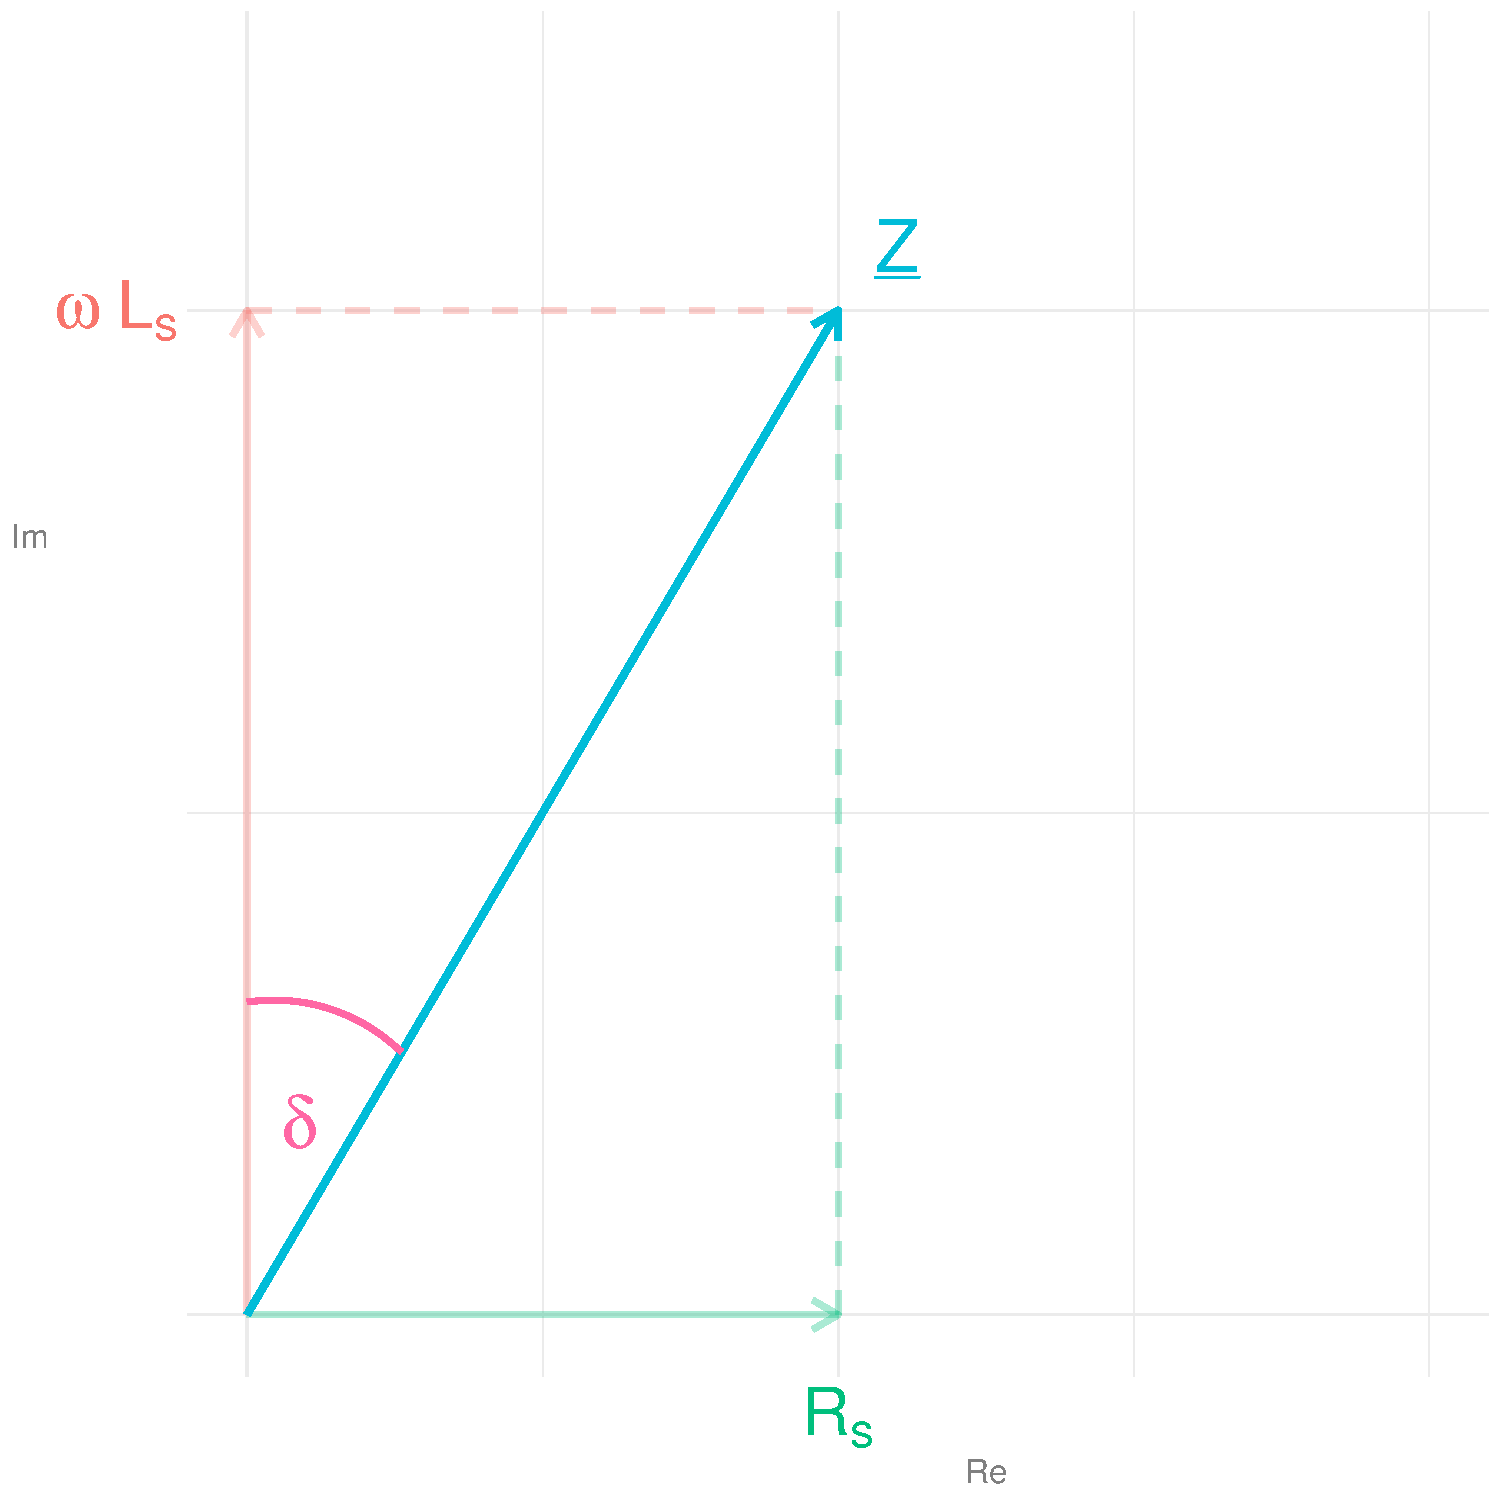
\includegraphics[scale=0.3819660112501051]{./R/2_1/ESBs_Spule.pdf}
    \end{center}

    Der Verlustwinkel $\delta$ ist der Winkel der Spulenimpedanz $\underline{Z}$ mit der imaginären Achse der gaußschen Zahlenebene. $\tan{\delta}$ wird auch Verlustfaktor $d$ genannt.

    $$\tan{\delta} = \frac{\omega L_s}{R_{sL}}$$

    Die Güte $Q$ der realen Induktivität ist demnach als Kehrwert des Verlustfaktors definiert:

    $$ Q_{Ls} = \frac{1}{\tan{\delta}} = \frac{R_{sL}}{\omega L_s}$$

    % Parallelmodell Spule
    \vspace{0.02128623625220817\paperheight}
    \begin{center}
    \large Parallelmodell

      \begin{circuitikz}

        \def\innerwidth{3}
        \def\innerheight{\innerwidth*0.3819660112501051}
        \def\klemmlength{\innerheight*0.6180339887498948}

        \draw (0,\innerheight/2)  to[R, l=$R_{pL}$] (\innerwidth,\innerheight/2);
        \draw (0,-\innerheight/2) to[L, l=$L_p$] (\innerwidth,-\innerheight/2);
        \draw (-\klemmlength,\klemmlength/4) to[short, o-] (0,\klemmlength/4);
        \draw (0,-\innerheight/2)  to[short] (0,\innerheight/2);
        \draw (\innerwidth,-\innerheight/2)  to[short] (\innerwidth,\innerheight/2);
        \draw (\innerwidth,\klemmlength/4) to[short, -o] (\innerwidth+\klemmlength,\klemmlength/4);

      \end{circuitikz}
    \end{center}

    \begin{center}
      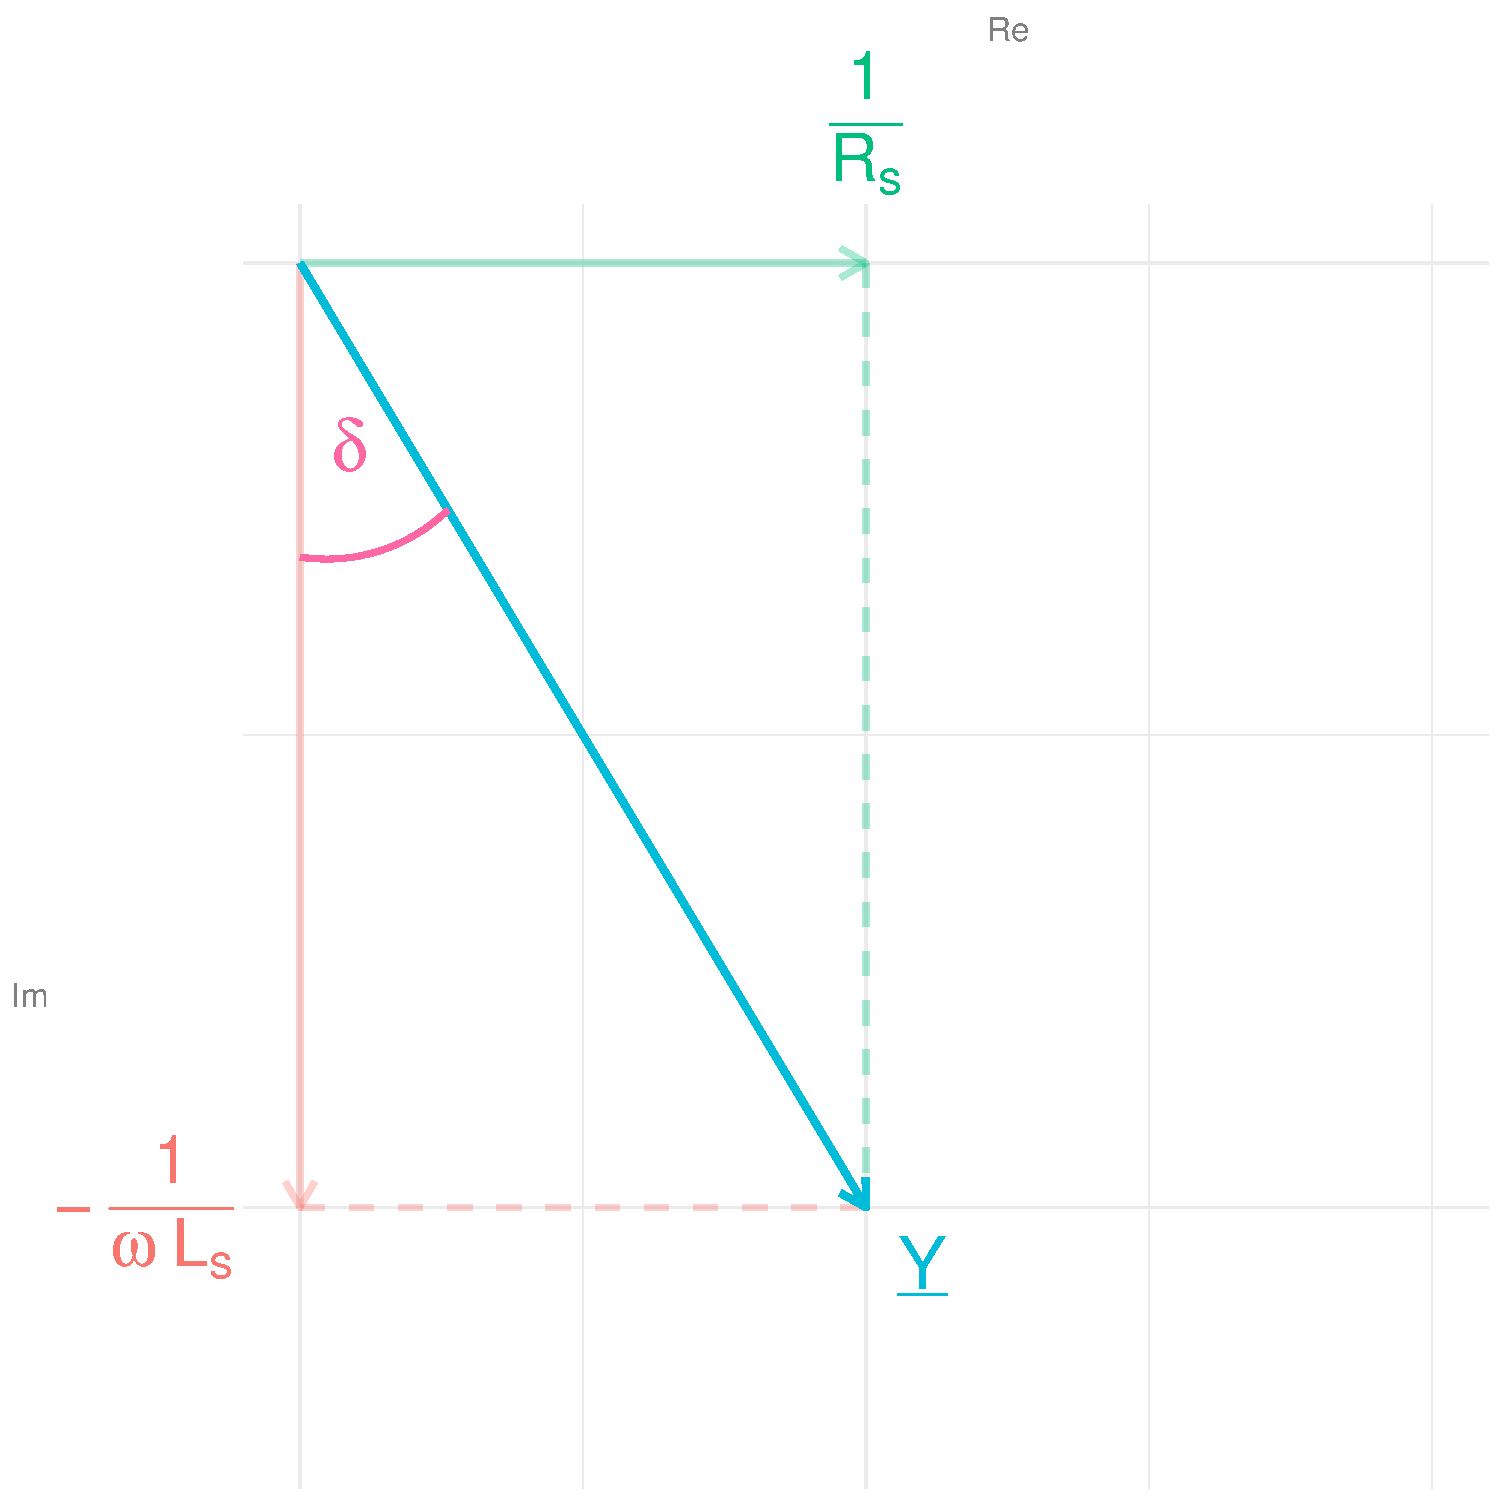
\includegraphics[scale=0.3819660112501051]{./R/2_1/ESBp_Spule.pdf}
    \end{center}

    Der Verlustwinkel $\delta$ ist der Winkel der Spulenadmittanz $\underline{Y}$ mit der imaginären Achse der gaußschen Zahlenebene (Betrag).

    $$\mid \tan{\delta} \mid=  \dfrac{\dfrac{1}{R_{pL}}}{\dfrac{1}{\omega L_p}} = \frac{\omega L_p}{R_{pL}}$$

    Kehrwert des Verlustfaktors:

    $$ Q_{Lp} = \frac{1}{\tan{\delta}} = \frac{R_{pL}}{\omega L_p}$$

    $$ Q_{Lp} = Q_{Ls} = \frac{R_{pL}}{\omega L_p} = \frac{\omega L_s}{R_{sL}}$$

    \pagebreak
    \subsubsection*{Kondensator}
    % Reihenmodell Kondensator
    \begin{center}

      \large Reihenmodell

        \begin{circuitikz}

          \draw (-0.3819660112501051,0) to[R, l=$R_{sC}$, o-] (1.6180339887498948,0);
          \draw (1.6180339887498948,0) to[C, l=$C_s$, -o] (1.6180339887498948*2+0.3819660112501051,0);

        \end{circuitikz}
      \end{center}

      \begin{center}
        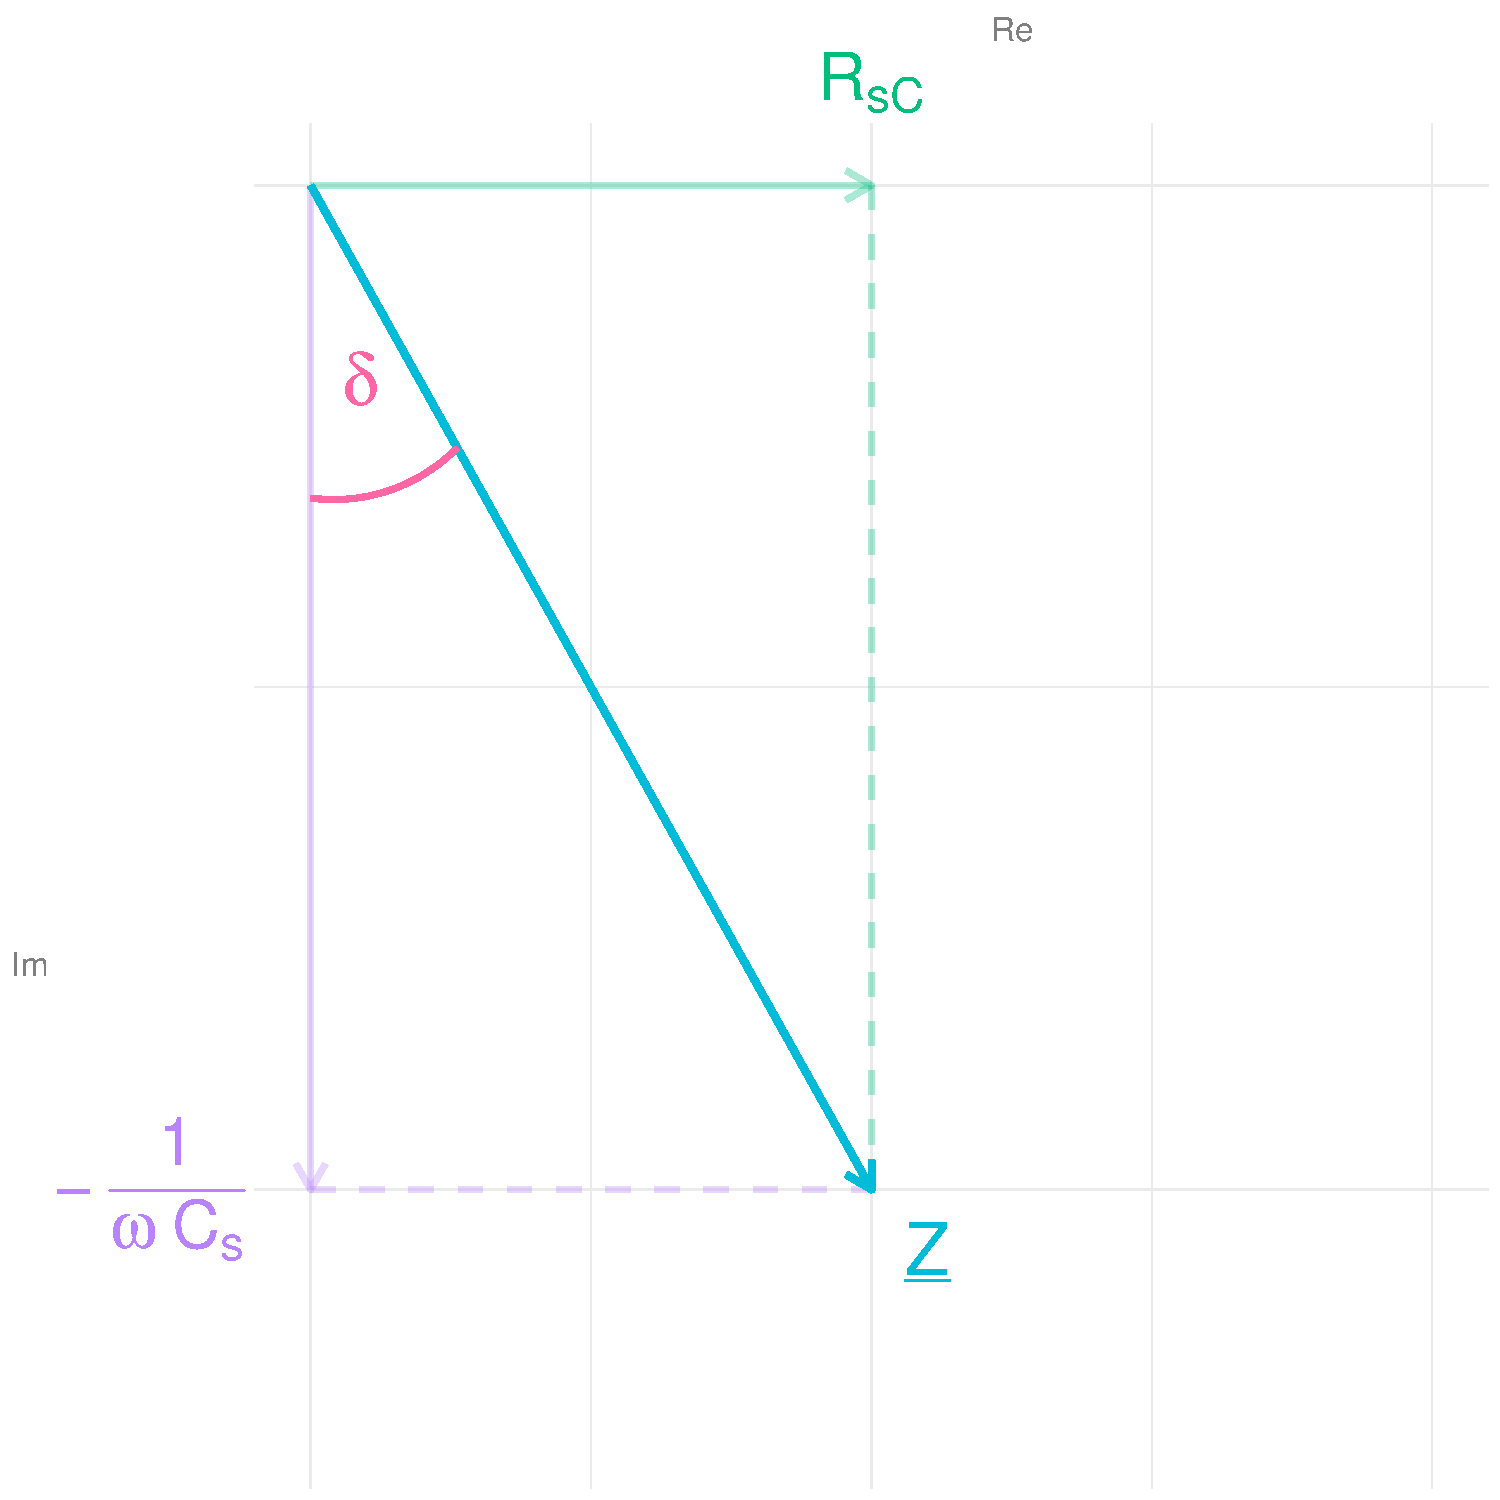
\includegraphics[scale=0.3819660112501051]{./R/2_1/ESBs_Kondensator.pdf}
      \end{center}

      Der Verlustwinkel $\delta$ ist der Winkel der Kondensatorimpedanz $\underline{Z}$ mit der imaginären Achse der gaußschen Zahlenebene (Betrag).

      $$\mid \tan{\delta} \mid = \dfrac{R_{sC}}{\dfrac{1}{\omega C_s}} = R_{sC} \cdot \omega C_s$$

      Somit ist die Kondensatorgüte des Reihenmodells:

      $$Q_{Cs}= \frac{1}{\tan{\delta}} = \frac{1}{R_{sC} \cdot \omega C_s}$$


    % Parallelmodell Kondensator
    \vspace{0.02128623625220817\paperheight}
    \begin{center}
    \large Parallelmodell

      \begin{circuitikz}

        \def\innerwidth{3}
        \def\innerheight{\innerwidth*0.3819660112501051}
        \def\klemmlength{\innerheight*0.6180339887498948}

        \draw (0,\innerheight/2)  to[R, l=$R_{pC}$] (\innerwidth,\innerheight/2);
        \draw (0,-\innerheight/2) to[C, l_=$C_p$] (\innerwidth,-\innerheight/2);
        \draw (-\klemmlength,\klemmlength/4) to[short, o-] (0,\klemmlength/4);
        \draw (0,-\innerheight/2)  to[short] (0,\innerheight/2);
        \draw (\innerwidth,-\innerheight/2)  to[short] (\innerwidth,\innerheight/2);
        \draw (\innerwidth,\klemmlength/4) to[short, -o] (\innerwidth+\klemmlength,\klemmlength/4);

      \end{circuitikz}
    \end{center}

    \begin{center}
      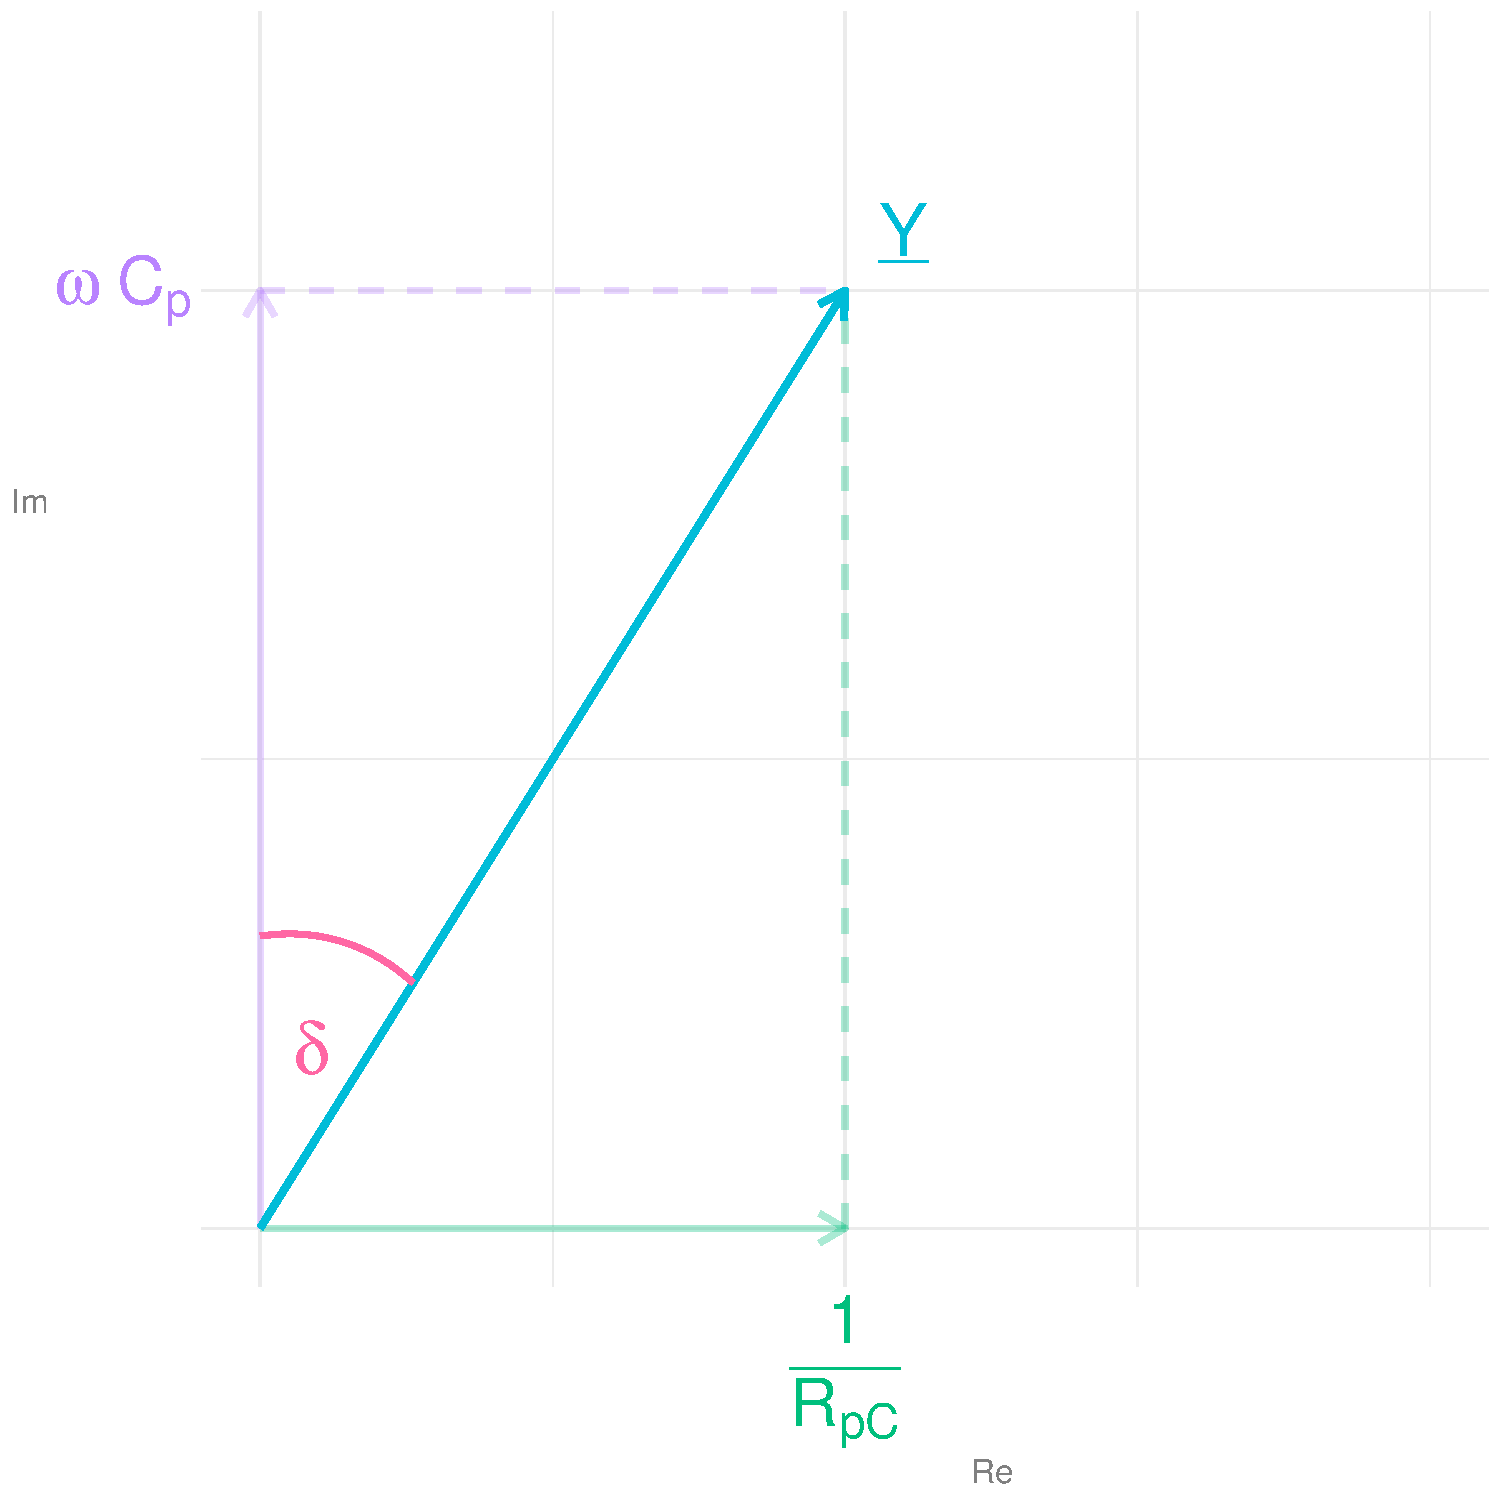
\includegraphics[scale=0.3819660112501051]{./R/2_1/ESBp_Kondensator.pdf}
    \end{center}

    Der Verlustwinkel $\delta$ ist der Winkel der Kondensatoradmittanz $\underline{Y}$ mit der imaginären Achse der gaußschen Zahlenebene.

    $$\tan{\delta} = \dfrac{\frac{1}{R_{pC}}}{\omega C_p} = \frac{1}{R_{pC} \cdot \omega C_p}$$

    Kehrwert des Verlustfaktors:

    $$ Q_{Cp} = \frac{1}{\tan{\delta}} = R_{pC} \cdot \omega C_p $$

    $$ Q_{Cs} = Q_{Cp} = \frac{1}{R_{sC} \cdot \omega C_s} = R_{pC} \cdot \omega C_p $$

  % 1.2
  \subsection{}

    \begin{center}
      \begin{circuitikz}

        \draw (-0.3819660112501051,0) to[R, l=$R_{s}$, o-] (1.6180339887498948,0);
        \draw (1.6180339887498948,0) to[L, l=$L$] (1.6180339887498948*2+0.3819660112501051,0)
        to[C, l=$C$, -o] (1.6180339887498948*3+0.3819660112501051,0);

      \end{circuitikz}
    \end{center}


    Gleichung (4):
      \begin{align*}
        \underline{Z} &= R_s + j(\omega L - \frac{1}{\omega C}) \tag{4´}\label{eq:4}\\
        &= R_s + j X\\
        &= \mid \underline{Z} \mid \cdot e^{j \phi_{\underline{Z}}}
      \end{align*}

    Gleichung (5):
      \begin{align*}
        \phi_{\underline{Z}} = \text{arg}(\underline{Z}) &= \arctan{\left(\frac{\omega L - \dfrac{1}{\omega C}}{R_s}\right)}\tag{5´}\label{eq:5}\\
        &= \arctan{\left(\frac{X}{R_s}\right)}
      \end{align*}

    Gleichung (6):
      \begin{align*}
        \mid \underline{Z} \mid = \sqrt{ R_s^2 + \left(\omega L - \frac{1}{\omega C}\right)^2 }\tag{6´}\label{eq:6}
      \end{align*}

    Gleichung (7):
      \begin{align*}
        \omega_0 = \frac{1}{\sqrt{LC}} \implies \omega_0 =\frac{1}{\sqrt{LC}} \tag{7´}\label{eq:7}
      \end{align*}

    Gleichung (8):
      \begin{align*}
        \underline{I} = \frac{\underline{U}}{\underline{Z}} \tag{8´}\label{eq:8}
      \end{align*}

    Gleichung (9):
     \begin{align*}
       \mid \underline{I} \mid &= \frac{\mid \underline{U} \mid}{\mid \underline{Z} \mid} \tag{9´}\label{eq:9}\\
       &= \frac{\mid \underline{U} \mid}{\sqrt{R_s^2 + \left( \omega L - \frac{1}{\omega C} \right)^2}}
     \end{align*}

    Gleichung (10):
     \begin{align*}
      \underline{I} = \underline{U} \cdot G_s = \frac{\underline{U}}{R_s} \tag{10´}\label{eq:10}\\
     \end{align*}

  % 1.3
  \subsection{}
    \subsubsection*{Reihenschwingkreis}

    \begin{center}
      \begin{circuitikz}

        \draw (-0.3819660112501051,0) to[R, l=$R_{s}$, o-] (1.6180339887498948,0);
        \draw (1.6180339887498948,0) to[L, l=$L_s$] (1.6180339887498948*2+0.3819660112501051,0)
        to[C, l=$C_s$, -o] (1.6180339887498948*3+0.3819660112501051,0);

      \end{circuitikz}
    \end{center}

    \vspace{0.013155617496424828\paperheight}
    \begin{center}
      \large Impedanzortskurve
    \end{center}

    $$\underline{Z} = R_s + j(\omega L_s - \frac{1}{\omega C_s})$$

    \begin{center}
      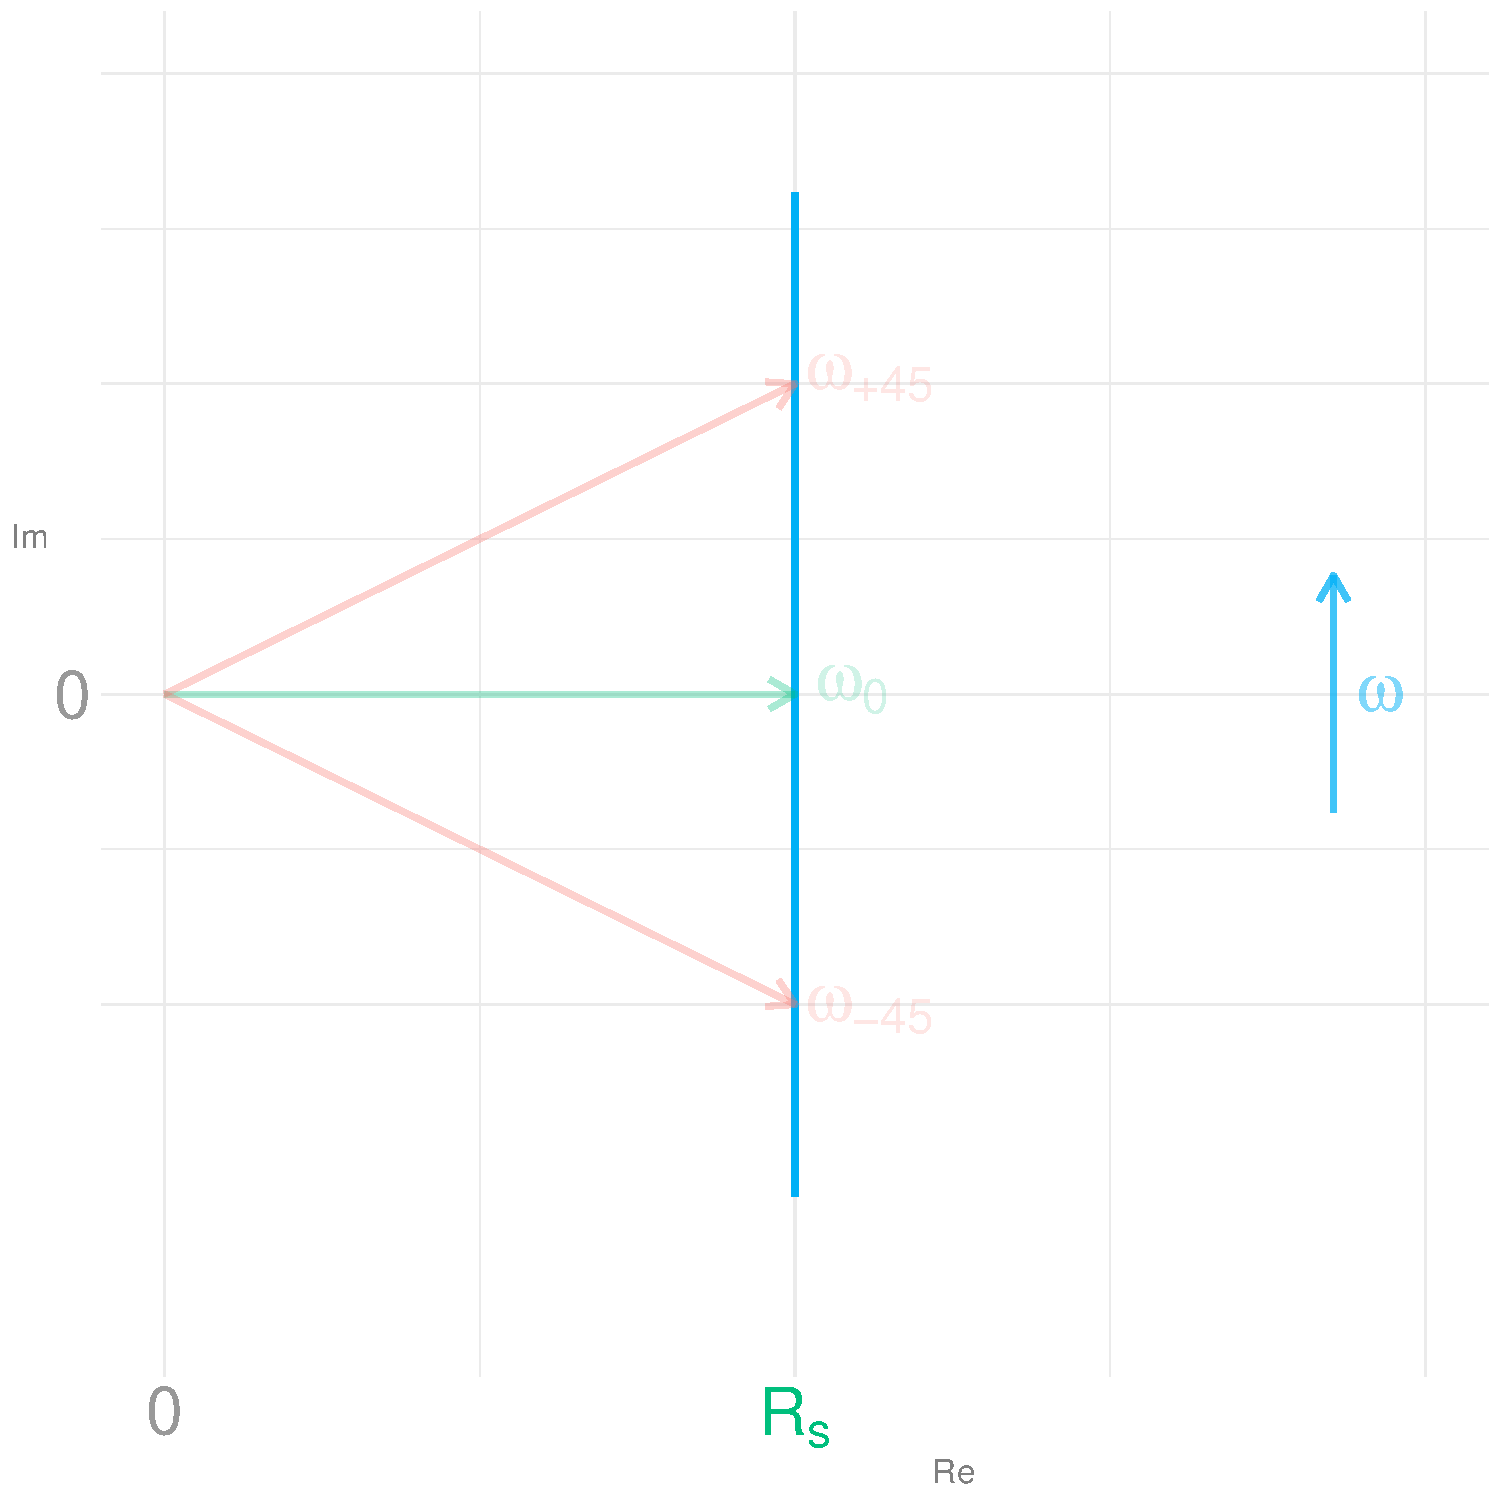
\includegraphics[scale=0.3819660112501051]{./R/2_3/SSK_Impedanz.pdf}
    \end{center}

    \begin{center}
      \large Admittanzortskurve
    \end{center}

    $$\underline{Y} = \frac{1}{R_s + j(\omega L_s - \frac{1}{\omega C_s})}$$

    \begin{center}
      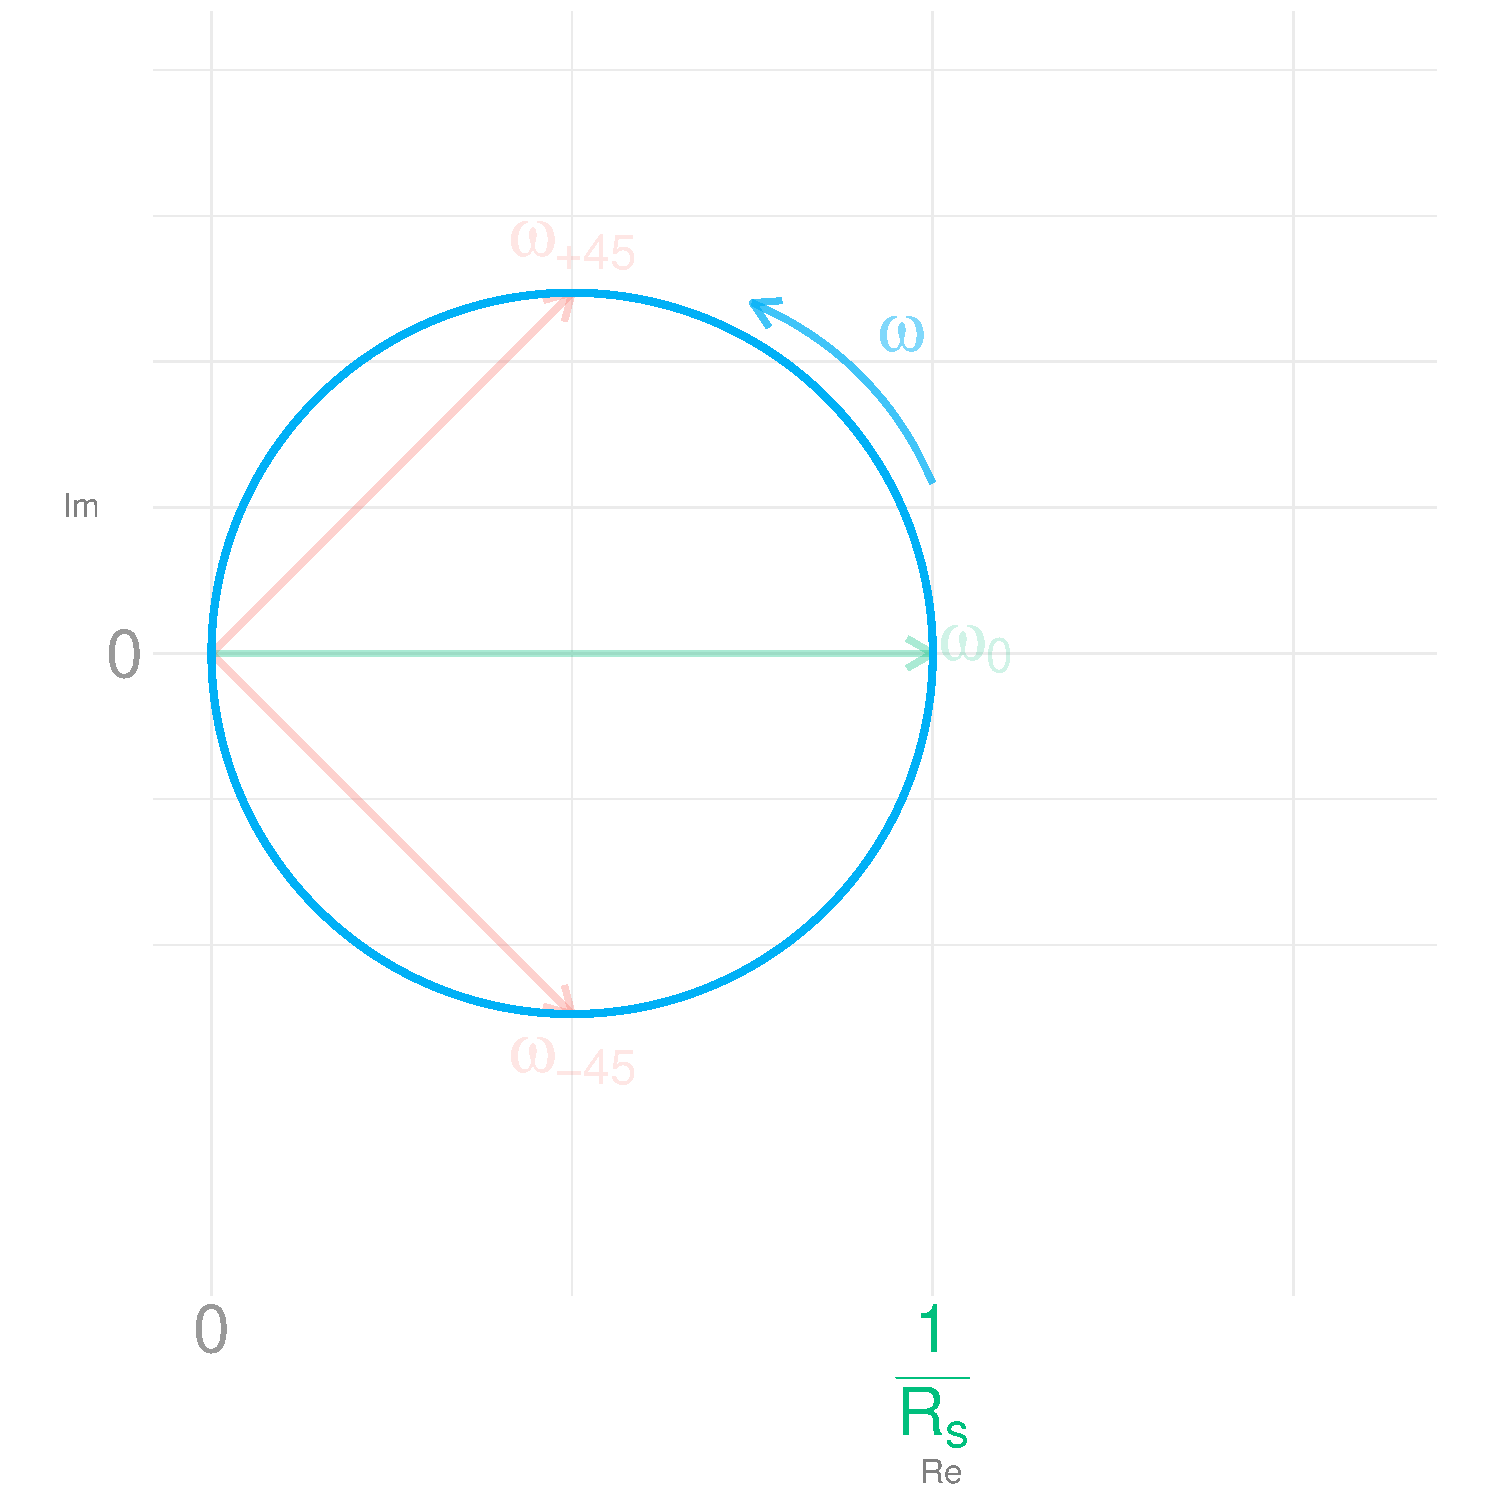
\includegraphics[scale=0.3819660112501051]{./R/2_3/SSK_Admittanz.pdf}
    \end{center}

    %%%%%%%%%%%%%%%%%%%%%%%%%%%%%%%%%%%%%
    \subsubsection*{Parallelschwingkreis}

    \begin{center}
      \begin{circuitikz}

        \def\innerwidth{3}
        \def\innerheight{\innerwidth*0.6180339887498948*1.6180339887498948}
        \def\klemmlength{\innerheight*0.3819660112501051}


        \draw (0,\innerheight/2)  to[R, l=$R_{p}$] (\innerwidth,\innerheight/2);
        \draw (0,0) to[L, l=$L_p$, *-*] (\innerwidth,0);
        \draw (0, -\innerheight/2) to[C, l=$C_p$] (\innerwidth, -\innerheight/2);

        %left short
        \draw (0, -\innerheight/2) to[short] (0, \innerheight/2);
        %right short
        \draw (\innerwidth, -\innerheight/2) to[short] (\innerwidth, \innerheight/2);

        \draw (-\klemmlength, \klemmlength/2) to[short, o-] (0,\klemmlength/2);
        \draw (\klemmlength+\innerwidth, \klemmlength/2) to[short, o-] (\innerwidth,\klemmlength/2);
      \end{circuitikz}
    \end{center}
    \vspace{0.013155617496424828\paperheight}
    \begin{center}
      \large Impedanzortskurve
      \vspace{-0.02128623625220817\paperheight}

      $$\underline{Z} = \frac{1}{\frac{1}{R_p} + j (\omega C_p - \frac{1}{\omega L_p}) }$$

      \begin{center}
        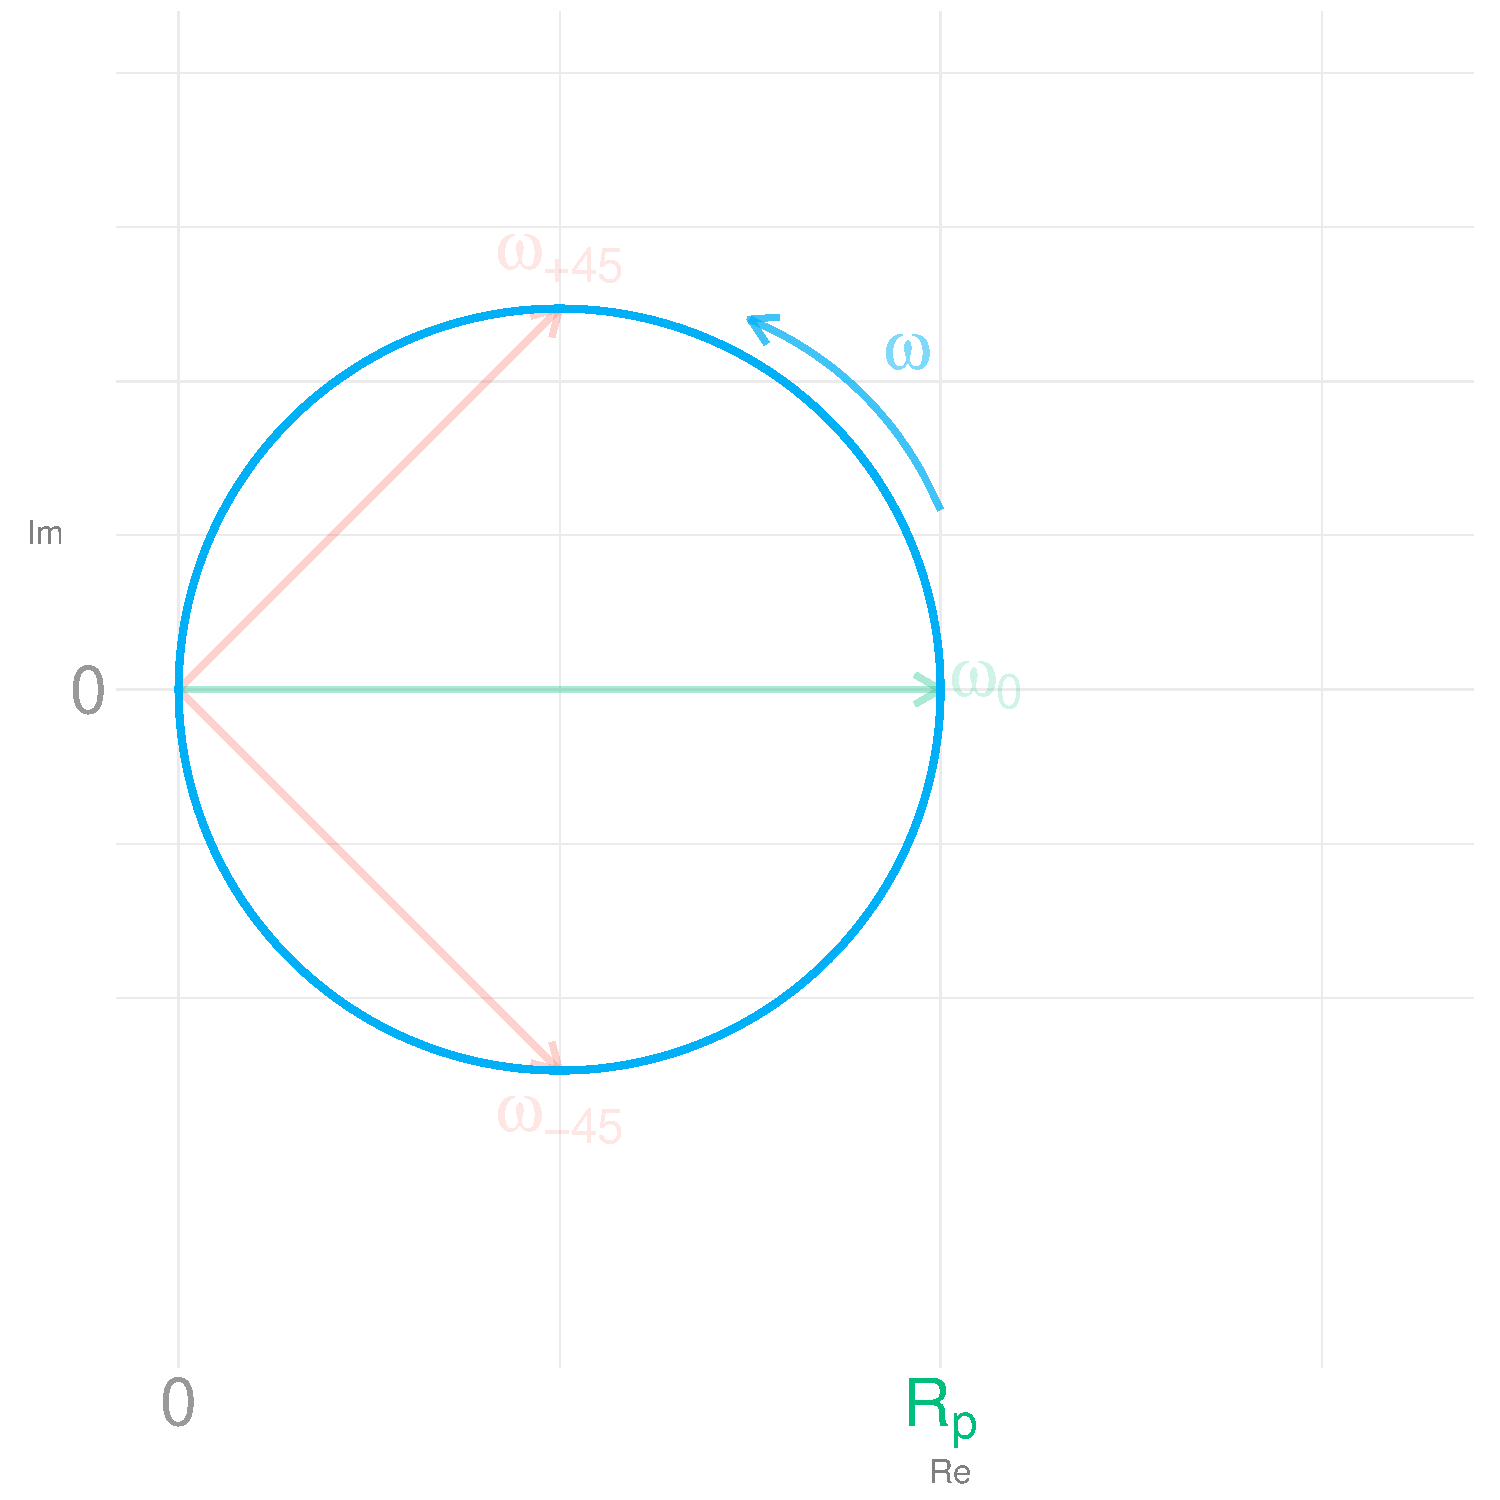
\includegraphics[scale=0.3819660112501051]{./R/2_3/PSK_Impedanz.pdf}
      \end{center}


    \end{center}

    \vspace{0.013155617496424828\paperheight}
    \begin{center}
      \large Admittanzortskurve
    \end{center}

    $$\underline{Y} = \frac{1}{R_p} + j (\omega C_p - \frac{1}{\omega L_p})$$


    \begin{center}
      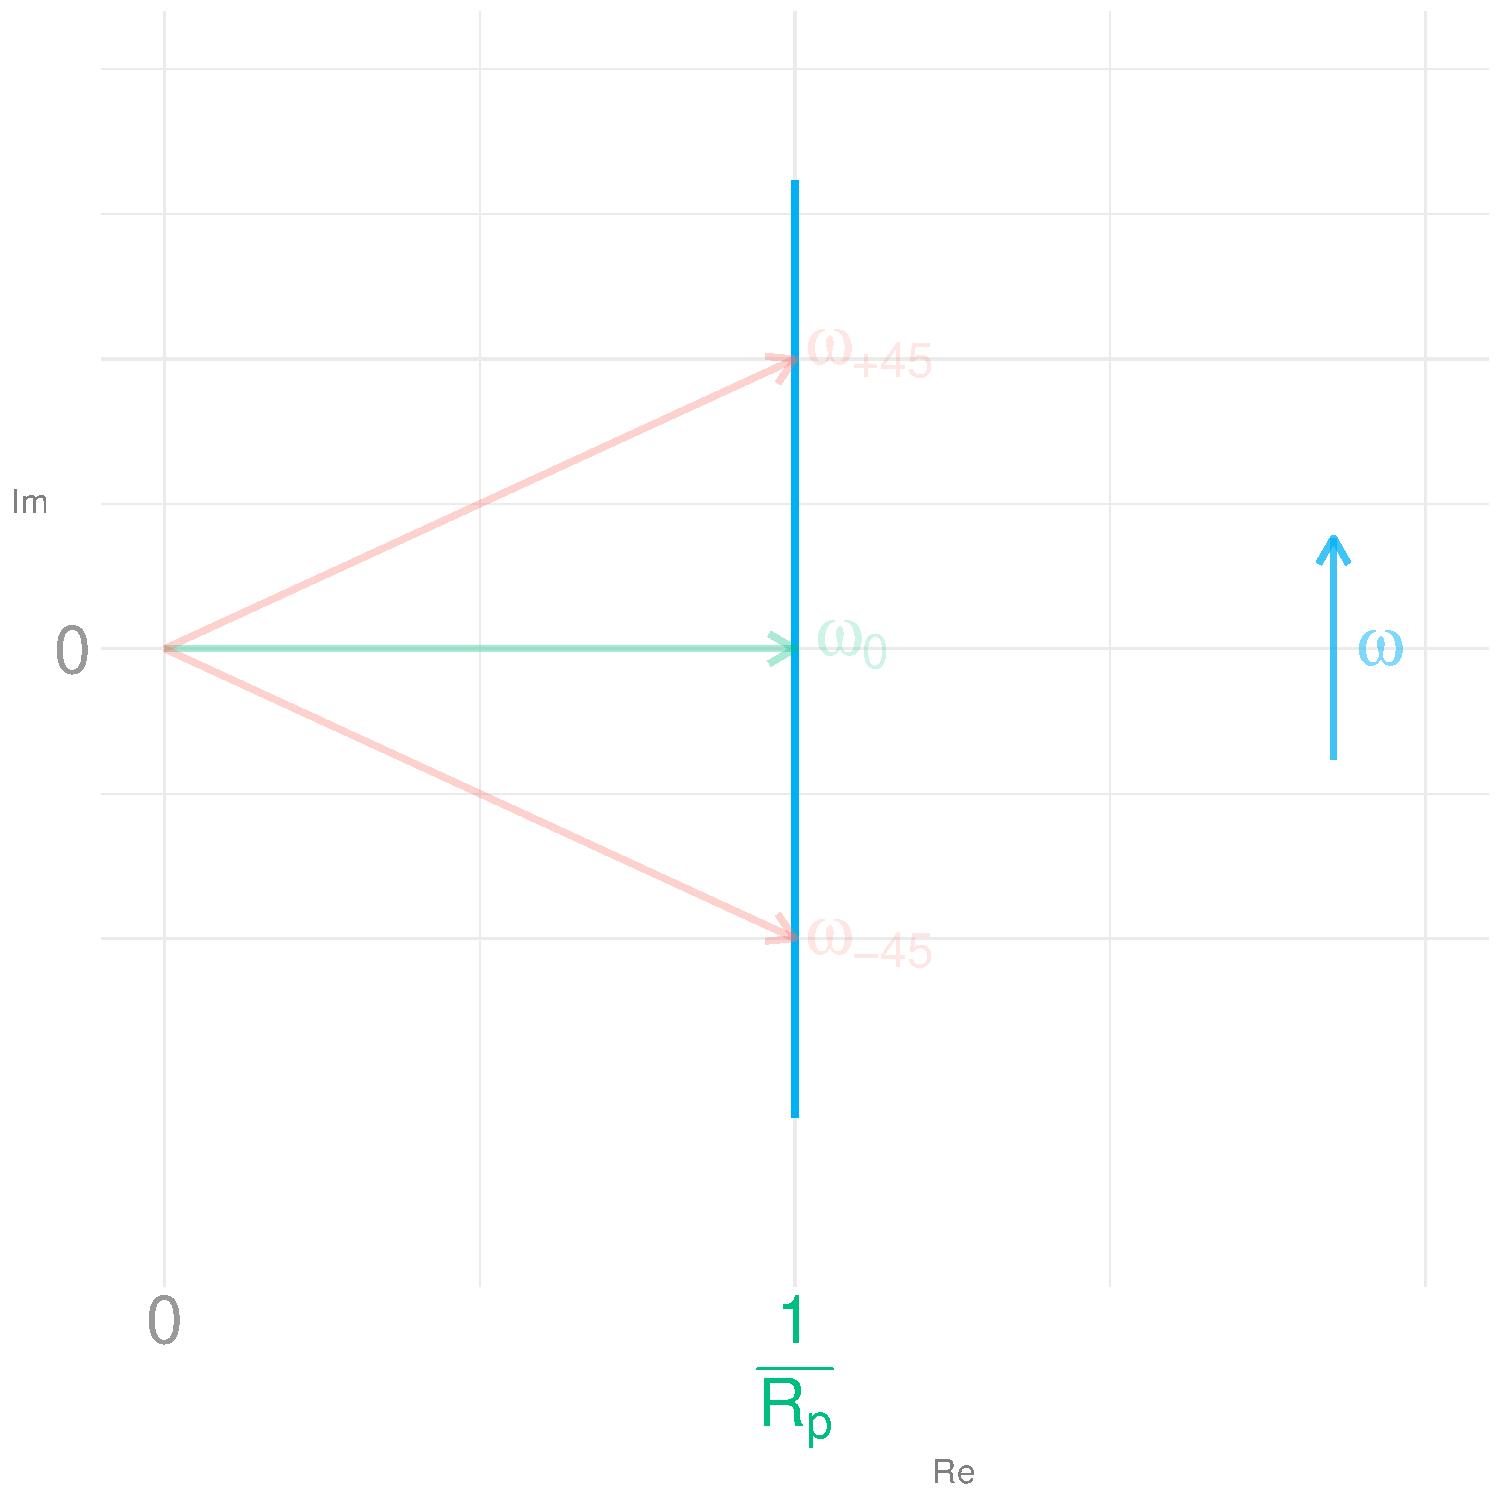
\includegraphics[scale=0.3819660112501051]{./R/2_3/PSK_Admittanz.pdf}
    \end{center}

  % 1.4
  \subsection{}
    % circuit
    \begin{center}
      \begin{circuitikz}

        \draw (0,0) to[R, l=$R_{sL}$] (2,0);
        \draw (2,0) to[L, l=$L$] (4,0);
        \draw (0,-1.6180339887498948) to[C, l=$C$] (4,-1.6180339887498948);

        \draw (0,0) to[short] (0,-1.6180339887498948);
        \draw (4,0) to[short] (4,-1.6180339887498948);

        \draw (-1, -0.3819660112501051) to[short, o-] (0,-0.3819660112501051);
        \draw (4, -0.3819660112501051) to[short, -o] (5,-0.3819660112501051);

      \end{circuitikz}
    \end{center}

    \begin{align*}
      \underline{Y} &= \frac{1}{R_{sL} + j \omega L} + j \omega C\\
                    &= \frac{R_{sL}}{R_{sL}^2 + \omega^2 L^2} + j \omega \left (C - \frac{ L}{ R_{sL}^2 + \omega^2 L^2 } \right )
    \end{align*}

    \begin{center}
      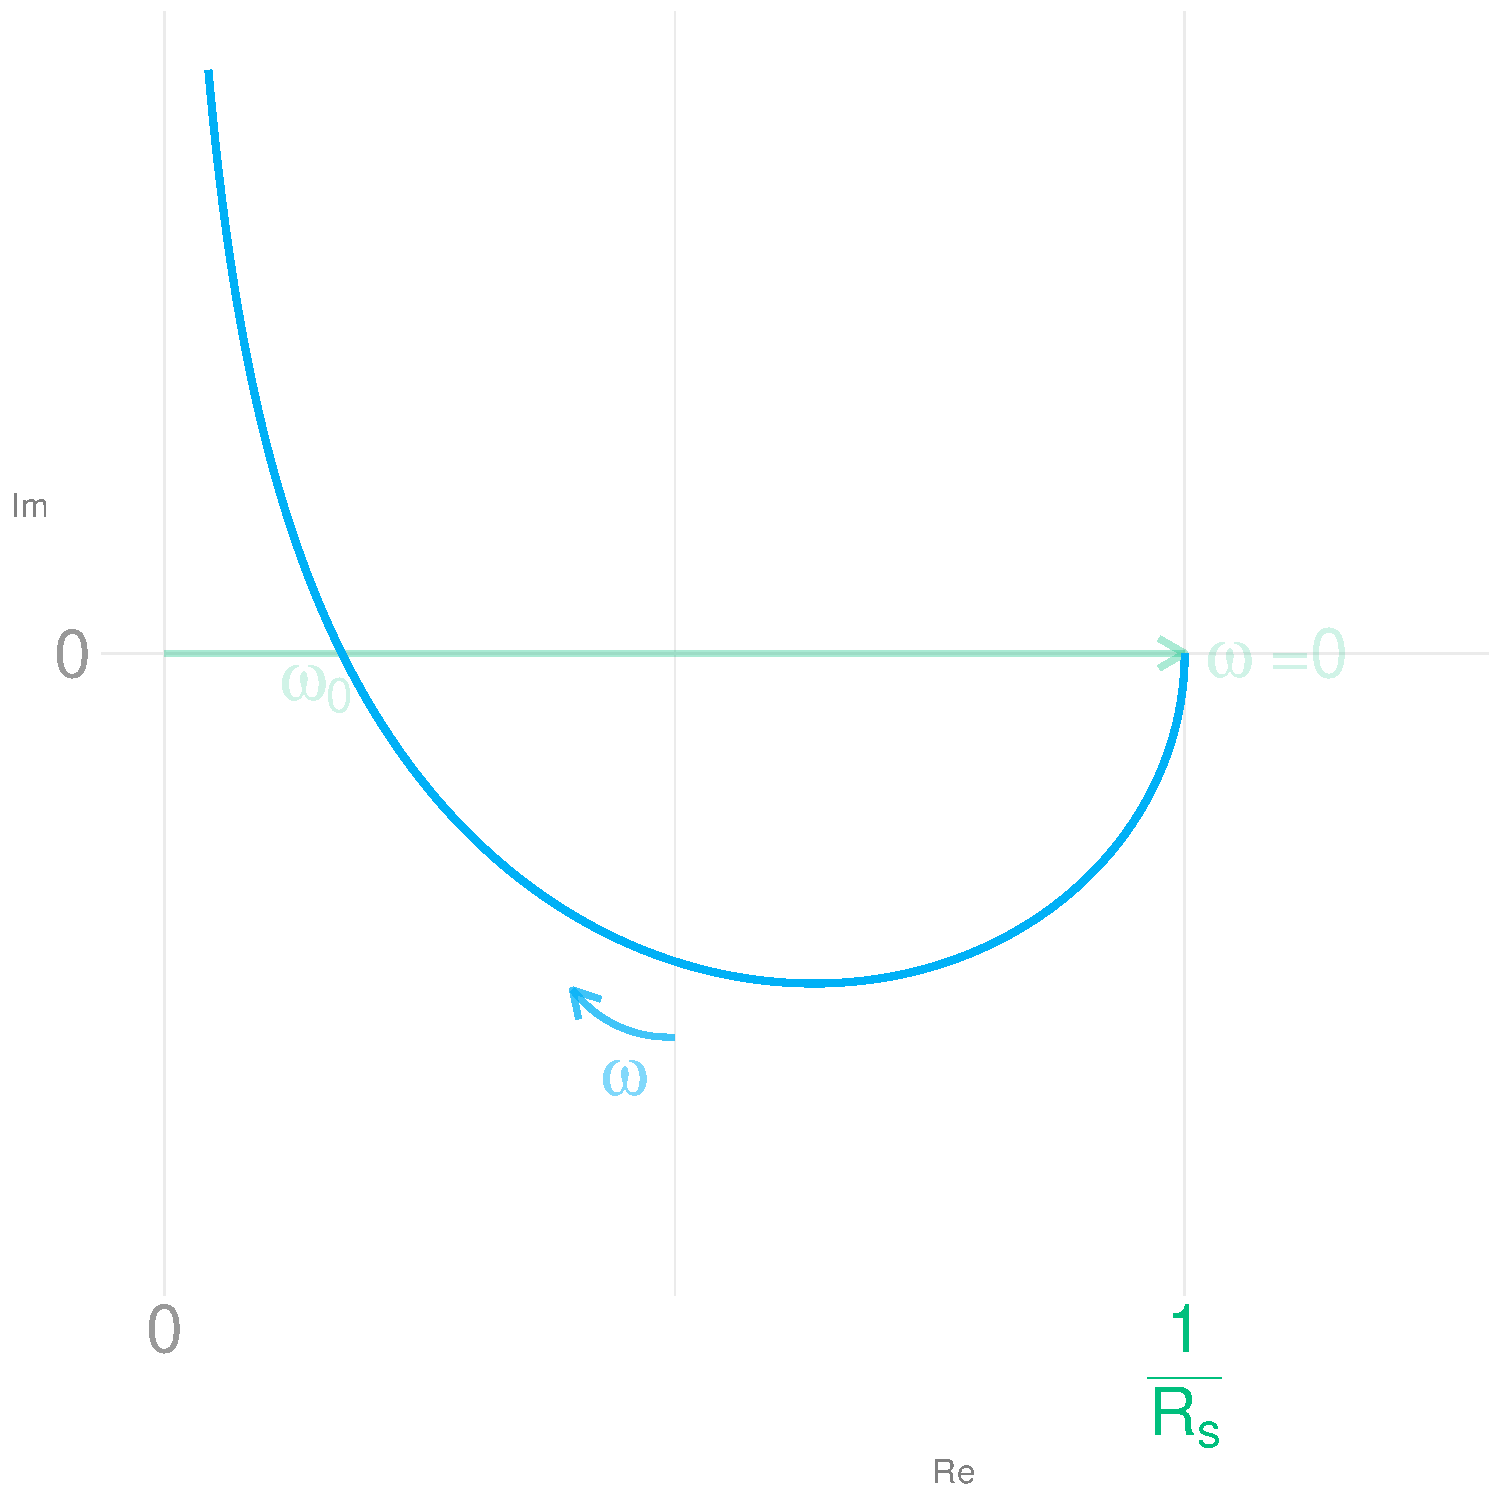
\includegraphics[scale=0.3819660112501051]{./R/2_4/2_4_OK.pdf}
    \end{center}

      \begin{gather*}
        \intertext{Resonanzfrequenz:}
        \text{Im}{(\underline{Y})} = 0\\
        \omega_0^{\text{´}} C - \frac{\omega_0^{\text{´}} L}{R_{sL}^2 + {\omega_0^{\text{´}}}^2 + L_s^2} = 0\\
        R_{sL}^2 \cdot C + {\omega_0^{\text{´}}}^2+L^2 \cdot C^2 = L\\
        \omega_0^{\text{´}} = \sqrt{ \underbrace{\frac{1}{LC}}_{\omega_0^2} - \frac{R_{sL}^2}{L^2} }\\
        \boxed{\omega_0^{\text{´}} = \omega_0 \sqrt{1-\frac{R_{sL}}{\omega_0^2 \cdot L^2} } = \omega_0 \sqrt{1-\frac{1}{Q_L^2}}}
      \end{gather*}

  % 1.5
  \subsection{}
    $$\omega_0 = \frac{1}{\sqrt{LC}} = \frac{1}{ \sqrt{1.3 \si{\henry} \cdot 22.5 \si{\nano\farad}} } = 5834.1 \,\ \si{\second}^{-1}$$

    $$\omega_0^{\text{´}} = \omega_0 \cdot \sqrt{1-\frac{R_{sL^2}}{\omega_0^2 \cdot L^2}} = 5834.1 \si{\second}^{-1} \cdot \sqrt{1-\frac{(100\si{\ohm})^2}{(5834.1 \si{\second}^{-1})^2 \cdot (1.3 \si{\henry})^2}}$$

    $$\omega_0^{\text{´}} = 5833.6 \,\ \si{\second}^{-1}$$

    \begin{center}
      $\implies$ geringe Differenz $\implies$ hohe Spulengüte
    \end{center}

    Zur Berechnung von Güte und Bandbreite wird der Schwingkreis in einen idealen Parallelschwingkreis umgewandelt:

    \begin{center}
      \begin{multicols}{3}[][1in]
        \raggedbottom

          \begin{circuitikz}
            \draw (-0.3819660112501051,0) to[R, l=$R_{sL}$, o-] (1.6180339887498948,0);
            \draw (1.6180339887498948,0) to[L, l=$L_s$, -o] (1.6180339887498948*2+0.3819660112501051,0);
          \end{circuitikz}

        $\implies$

        \begin{circuitikz}

          \def\innerwidth{3}
          \def\innerheight{\innerwidth*0.3819660112501051}
          \def\klemmlength{\innerheight*0.6180339887498948}

          \draw (0,\innerheight/2)  to[R, l=$R_{p}$] (\innerwidth,\innerheight/2);
          \draw (0,-\innerheight/2) to[L, l=$L_p$] (\innerwidth,-\innerheight/2);
          \draw (-\klemmlength,\klemmlength/4) to[short, o-] (0,\klemmlength/4);
          \draw (0,-\innerheight/2)  to[short] (0,\innerheight/2);
          \draw (\innerwidth,-\innerheight/2)  to[short] (\innerwidth,\innerheight/2);
          \draw (\innerwidth,\klemmlength/4) to[short, -o] (\innerwidth+\klemmlength,\klemmlength/4);

        \end{circuitikz}

      \end{multicols}
    \end{center}

    \begin{align*}
      \underline{Y}_s &= \underline{Y}_p\\
      \frac{1}{R_s + j \omega_0 L_s} &= \frac{1}{R_p}-j\frac{1}{\omega_0 L_p}\\
      %\intertext{\small Trennung in Real- und Imaginärteil zum Vergleich:}
      \frac{R_s}{R_s^2+\omega_0^2 L_s^2}-j\frac{\omega_0 L_s}{R_s^2 L_s + \omega_0^2 L_s} &= \frac{1}{R_p}-j\frac{1}{\omega_0 L_p}
    \end{align*}

    \small Realteilvergleich:
    \begin{gather*}
      R_{p} = 1+\frac{\omega_0^2 L_s^2}{R_s^2} = 1 + Q_L^2
    \end{gather*}
    \small Imaginärteilvergleich:
    \begin{gather*}
      L_{p} = L_s\left( 1+ \frac{R_{s}^2}{\omega_0^2 L_s^2} \right) = 1+ \frac{1}{Q_L^2}
    \end{gather*}

    $$R_{p} = 575.3 \,\ \si{\kilo\ohm}\text{,} \,\ L_p = 1.30023 \,\ \si{\henry} \approx L_s$$

  % 1.6
  \subsection{}
    \begin{center}
      \large Stromspeisung
    \end{center}

    \begin{center}
      \begin{circuitikz}

        \draw (0.3819660112501051, 1.618/2) to[short] (0.3819660112501051 + 1, 1.618/2);
        \draw (0.3819660112501051, -1.618/2) to[short] (0.3819660112501051 + 1, -1.618/2);

        \draw (-1.618, -1.618/2) to[ioosource] (-1.618, 1.618/2)
                                 to[short, -o, i=$\underline{I}_0$] (0.3819660112501051, 1.618/2);
        \draw (-1.618, -1.618/2) to[short, -o] (0.3819660112501051, -1.618/2);

        \draw (0.3819660112501051 + 1, 1.618/2) to[R, l=$\underline{Z}_{SK}$] (0.3819660112501051 + 1, -1.618/2);

        \draw[draw=black] (0.3819660112501051 + 0.23606797749978964, 1.618) rectangle ++(0.3819660112501051*6, -1.618*2);

        \node[draw] at (0.3819660112501051*6-0.05572809000084119, -1.618/2-0.1458980337503154) {SK};
      \end{circuitikz}
    \end{center}

    $$\underline{U} = \underline{Z}_{SK} \cdot \underline{I}_0, \,\ \text{ $\underline{I}_0 =$ konst.} \implies \underline{U} \sim \underline{Z}_{SK}$$

    \begin{center}
      \large Spannungsspeisung
    \end{center}

    \begin{center}
      \begin{circuitikz}

        \draw (0.3819660112501051, 1.618/2) to[short] (0.3819660112501051 + 1, 1.618/2);
        \draw (0.3819660112501051, -1.618/2) to[short] (0.3819660112501051 + 1, -1.618/2);

        \draw (-1.618, 1.618/2) to[vsourcesin, v_=$\underline{U}_0$] (-1.618, -1.618/2);
        \draw (-1.618, 1.618/2) to[short, -o] (0.3819660112501051, 1.618/2);
        \draw (-1.618, -1.618/2) to[short, -o] (0.3819660112501051, -1.618/2);

        \draw (0.3819660112501051 + 1, 1.618/2) to[R, l=$\underline{Z}_{SK}$] (0.3819660112501051 + 1, -1.618/2);

        \draw[draw=black] (0.3819660112501051 + 0.23606797749978964, 1.618) rectangle ++(0.3819660112501051*6, -1.618*2);

        \node[draw] at (0.3819660112501051*6-0.05572809000084119, -1.618/2-0.1458980337503154) {SK};
      \end{circuitikz}
    \end{center}

    $$\underline{I} = \underline{U} \cdot \underline{Y}_{SK}, \,\ \text{ $\underline{U}_0 =$ konst.} \implies \underline{I} \sim \underline{Y}_{SK}$$

  % 1.7
  \subsection{}

    \begin{center}
      \large Spannungsüberhöhung\\
      \small (Nur im Reihenschwingkreis)
    \end{center}

    \begin{center}
      \begin{circuitikz}
        \draw (-0.3819660112501051, 0) to[short, o-] (0,0)
                                       to[R, l=$R_s$, v=$\underline{U}_{R_s}$] (2,0)
                                       to[L, l=$L_s$, v=$\underline{U}_{L_s}$] (4,0)
                                       to[C, l=$C_s$, v=$\underline{U}_{C_s}$] (6,0)
                                       to[short, -o] (6+0.3819660112501051,0);
      \end{circuitikz}
    \end{center}

      $R_s$:
      \begin{gather*}
        \underline{U}_{R_s} = \frac{\underline{U} \cdot R_s}{R_s + j\left( \omega L_s - \frac{1}{\omega C_s} \right)}
      \end{gather*}
      \indent $L_s$:
      \begin{gather*}
        \underline{U}_{L_s} = \frac{\underline{U} \cdot j \omega L_s}{ R_s + j\left( \omega L_s - \frac{1}{\omega C_s} \right)}
      \end{gather*}
      \indent $C_s$:
      \begin{gather*}
        \underline{U}_{C_s} = \frac{\underline{U}}{ j \omega C_s\left(R_s + j\left( \omega L_s - \frac{1}{\omega C_s} \right)\right)}
      \end{gather*}

      bei $\omega = \omega_0$:

      \begin{align*}
        \underline{U}_{R_s} &= \frac{\underline{U} \cdot R_s}{R_s} = \underline{U}\\
        \underline{U}_{L_s} &= j \underline{U} \cdot \frac{ \omega_0 L_s}{R_s} = j \underline{U} \cdot Q_L\\
        \underline{U}_{C_s} &= -j \underline{U} \cdot \frac{1}{ \omega_0 C_s R_s}
      \end{align*}

      Beträge bei $\omega_0$:

      \begin{align*}
        \hat{U}_{R_s} &= \hat{U}\\
        \hat{U}_{L_s} &= Q_L \cdot \underline{U}\\
        \hat{U}_{C_s} &= Q_C \cdot \underline{U}
      \end{align*}

      %%%%%%%%%%%%%%%%%%%%%%%%%%%%%%%%%%%%%%%%%%%%
    \begin{center}
      \large Stromüberhöhung\\
      \small (Nur im Parallelschwingkreis)
    \end{center}

    \begin{center}
      \begin{circuitikz}
        \def\innerwidth{3}
        \def\innerheight{\innerwidth*0.6180339887498948*1.6180339887498948}
        \def\klemmlength{\innerheight*0.3819660112501051}


        \draw (0,\innerheight/2)  to[R, l=$R_{p}$, i=$\underline{I}_{R_p}$] (\innerwidth,\innerheight/2);
        \draw (0,0) to[L, l=$L_p$, i=$\underline{I}_{L_p}$, *-*] (\innerwidth,0);
        \draw (0, -\innerheight/2) to[C, l=$C_p$, i=$\underline{I}_{C_p}$] (\innerwidth, -\innerheight/2);

        %left short
        \draw (0, -\innerheight/2) to[short] (0, \innerheight/2);
        %right short
        \draw (\innerwidth, -\innerheight/2) to[short] (\innerwidth, \innerheight/2);

        \draw (-\klemmlength, \klemmlength/2) to[short, o-] (0,\klemmlength/2);
        \draw (\klemmlength+\innerwidth, \klemmlength/2) to[short, o-] (\innerwidth,\klemmlength/2);
      \end{circuitikz}
    \end{center}

    $R_p$:
    \begin{gather*}
      \underline{I}_{R_p} = \frac{\underline{I} \cdot \frac{1}{R_p}}{\frac{1}{R_p} + j\left( \omega C_p - \frac{1}{\omega L_p} \right)}
    \end{gather*}
    \indent $L_p$:
    \begin{gather*}
      \underline{I}_{L_p} = \frac{\underline{I}}{ j \omega L_p \left(\frac{1}{R_p} + j\left( \omega C_p - \frac{1}{\omega L_p} \right)\right)}
    \end{gather*}
    \indent $C_p$:
    \begin{gather*}
      \underline{I}_{C_p} = \frac{\underline{I} \cdot j \omega C_p}{ \frac{1}{R_p} + j\left( \omega C_p - \frac{1}{\omega L_p} \right)}
    \end{gather*}

    bei $\omega = \omega_0$:

    \begin{align*}
      \underline{I}_{R_p} &= \underline{I}\\
      \underline{I}_{L_p} &= j \underline{I} \cdot \frac{R_p}{\omega_0 L_p} = j \underline{I} \cdot Q_L\\
      \underline{I}_{C_p} &= -j \underline{I} \cdot \omega_0 R_p C_p = j \underline{I} \cdot Q_C
    \end{align*}

    Beträge bei $\omega_0$:

    \begin{align*}
      \hat{I}_{R_p} &= \hat{I}\\
      \hat{I}_{L_p} &= Q_L \cdot \underline{I}\\
      \hat{I}_{C_p} &= Q_C \cdot \underline{I}
    \end{align*}

    Die Strom- bzw. Spannungsüberhöhungen betragen demnach bei Resonanz das $Q_{L/C}$-fache der Quellgrößen.

  % 1.8
  \subsection{}
  \begin{gather*}
    \omega_0 = \frac{1}{\sqrt{LC}} = \frac{1}{\sqrt{0.1 \si{\henry} \cdot 100 \si{\nano\farad}}} = 10000 \,\ \si{\second}^{-1} \implies f_0 = 1.592 \,\ \si{\kilo\hertz}
  \end{gather*}

  \vspace{0.013155617496424828\paperheight}

  \pagebreak
  \begin{multicols*}{2}


    \begin{center}
      Spule\\

        \begin{circuitikz}
          \draw (-0.3819660112501051,0) to[R, l=$R_{sL}$, o-] (1.6180339887498948,0);
          \draw (1.6180339887498948,0) to[L, l=$L_s$, -o] (1.6180339887498948*2+0.3819660112501051,0);
        \end{circuitikz}

      \begin{gather*}
        Q_L = \frac{\omega_0 L_s}{R_{sL}}\\
        R_{sL} = \frac{\omega_0 L_s}{Q_L} = 20 \,\ \si{\ohm}
      \end{gather*}

      \vspace{0.013155617496424828\paperheight}

      \begin{circuitikz}

        \def\innerwidth{3}
        \def\innerheight{\innerwidth*0.3819660112501051}
        \def\klemmlength{\innerheight*0.6180339887498948}

        \draw (0,\innerheight/2)  to[R, l=$R_{pL}$] (\innerwidth,\innerheight/2);
        \draw (0,-\innerheight/2) to[L, l=$L_p$] (\innerwidth,-\innerheight/2);
        \draw (-\klemmlength,\klemmlength/4) to[short, o-] (0,\klemmlength/4);
        \draw (0,-\innerheight/2)  to[short] (0,\innerheight/2);
        \draw (\innerwidth,-\innerheight/2)  to[short] (\innerwidth,\innerheight/2);
        \draw (\innerwidth,\klemmlength/4) to[short, -o] (\innerwidth+\klemmlength,\klemmlength/4);
      \end{circuitikz}

      \begin{gather*}
        Q_L = \frac{R_{pL}}{\omega_0 L_p}\\
        R_{pC} = Q_L \cdot \omega_0 L_p = 50 \,\ \si{\kilo\ohm}
      \end{gather*}

    \end{center}

    \vfill\columnbreak
    %%%%%%%%%%%%%%%%%%%%%%%
    \begin{center}
      Kondensator\\
      \begin{circuitikz}
        \draw (-0.3819660112501051,0) to[R, l=$R_{sC}$, o-] (1.6180339887498948,0);
        \draw (1.6180339887498948,0) to[C, l=$C_s$, -o] (1.6180339887498948*2+0.3819660112501051,0);
      \end{circuitikz}

      \begin{gather*}
        Q_C = \frac{1}{\omega_0 R_{sC} C_s}\\
        R_{sC} = \frac{1}{\omega_0 Q_C C_s} = 3.3 \,\ \si{\ohm}
      \end{gather*}

      \vspace{0.013155617496424828\paperheight}

      \begin{circuitikz}

        \def\innerwidth{3}
        \def\innerheight{\innerwidth*0.3819660112501051}
        \def\klemmlength{\innerheight*0.6180339887498948}

        \draw (0,\innerheight/2)  to[R, l=$R_{pC}$] (\innerwidth,\innerheight/2);
        \draw (0,-\innerheight/2) to[C, l_=$C_p$] (\innerwidth,-\innerheight/2);
        \draw (-\klemmlength,\klemmlength/4) to[short, o-] (0,\klemmlength/4);
        \draw (0,-\innerheight/2)  to[short] (0,\innerheight/2);
        \draw (\innerwidth,-\innerheight/2)  to[short] (\innerwidth,\innerheight/2);
        \draw (\innerwidth,\klemmlength/4) to[short, -o] (\innerwidth+\klemmlength,\klemmlength/4);

      \end{circuitikz}

      \begin{gather*}
        Q_C = \omega_0 R_{pC} C_p\\
        R_{pC} = \frac{Q_C}{\omega_0 C_p} = 300 \,\ \si{\kilo\ohm}
      \end{gather*}

    \end{center}
  \end{multicols*}

  \begin{gather*}
    Q_{SK} = \frac{1}{\dfrac{1}{Q_c}+\dfrac{1}{Q_L}} = \frac{Q_C \cdot Q_L}{Q_C + Q_L}\\
    Q_{SK} = \frac{300}{7} \approx 42.86
  \end{gather*}

  \begin{gather*}
    B_{\omega} = \frac{\omega_0}{Q_{SK}} = \frac{10000 \si{\second}^{-1}}{42.86} = 232.3 \,\ \si{\second}^{-1}\\
    B_{f} = \frac{223.2\si{\second}^{-1}}{2\pi} = 37.14 \,\ \si{\hertz}
  \end{gather*}


  % 1.9
  \subsection{}

\section{Versuchsaufgaben}


\end{document}
